\documentclass{article}
\usepackage{malmacros}
\begin{document}

\section{Compression}
In this section, the ability to compress data and train on this data is explored, using PCA by using SVD decomposition. A data set is compressed and trained upon to investigate how well the classifier will perform and how fast. It will be looked into how noise from a data set can be reduced. Lastly it will be attempted to use 'PCA -> t-SNE' components to train and test a data set. 

\subsection{Speed}

\begin{pyminted}
from six.moves import urllib
from sklearn.datasets import fetch_openml
from sklearn.model_selection import train_test_split

mnist = fetch_openml('mnist_784', version=1, cache=True)

X = mnist["data"]
y = mnist["target"]

X_train, X_test, y_train, y_test = train_test_split(X, y)
\end{pyminted}

\begin{pyminted}
from sklearn.linear_model import LogisticRegression
import time

logisticRegr = LogisticRegression(solver = 'lbfgs',max_iter = 1000, multi_class = 'multinomial')

time_start = time.time()
logisticRegr.fit(X_train, y_train)
print('logisticRegr done! Time elapsed: {} seconds'.format(time.time()-time_start))

logisticRegr.score(X_test, y_test)
\end{pyminted}
\begin{pyconsole}
logisticRegr done! Time elapsed: 49.92672157287598 seconds
0.9128
\end{pyconsole}

\subsubsection{Achieving speed by using PCA for compression}
Using PCA for compression t is possible to achieve much higher speed for fitting the model to the compressed data. By only compressing the MNIST data to 95\% of its original size it was possible to go from fitting the data in 49.93 seconds to only 18.15 seconds. This even resulted in a slightly higher score for logistic regression model.

\begin{pyminted}
from sklearn.linear_model import LogisticRegression
import time
from sklearn.decomposition import PCA

logisticRegr = LogisticRegression(solver = 'lbfgs',max_iter = 1000, multi_class = 'multinomial')

# Compress X. Transform X_test.. like: pca.transform(X_test). This was done previously.
pca = PCA(0.95, random_state=42)
X_train_reduced = pca.fit_transform(X_train) #compress
X_test_reduced = pca.transform(X_test)

time_start = time.time()
logisticRegr.fit(X_train_reduced, y_train)

print('Version 2: logisticRegr done! Time elapsed: {} seconds'.format(time.time()-time_start))

logisticRegr.score(X_test_reduced, y_test)
\end{pyminted}
\begin{pyconsole}
Version 2: logisticRegr done! Time elapsed: 18.150802850723267 seconds

0.9198857142857143
\end{pyconsole}


\section{Noise reduction}

A possible solutions to overfitting is using noise reduction. This can involve removing outliers. It is possible to use noise reduction using compression with PCA to recover data to being closer to its original noiseless state.

\begin{pyminted}
from sklearn.datasets import fetch_openml

mnist = fetch_openml('mnist_784', version=1, cache=True)
\end{pyminted}
\begin{pyminted}
from sklearn.model_selection import train_test_split

X = mnist["data"]
y = mnist["target"]

X_train, X_test, y_train, y_test = train_test_split(X, y)
\end{pyminted}
\begin{pyminted}
#generate noisy data
from sklearn.model_selection import train_test_split
np.random.seed(42)
X_noisy = np.random.normal(X, 200)
X_noisy_train, X_noisy_test, y_noisy_train, y_noisy_test, = train_test_split(X_noisy, y, random_state=42)

plt.figure(figsize=(14, 8))
plt.subplot(121)
plot_digits(X_train[::2100])
plt.title("Original", fontsize=16)
plt.subplot(122)
plot_digits(X_noisy_train[::2100])
plt.title("Noisy", fontsize=16)
\end{pyminted}

\begin{figure}[H]
  \centering
    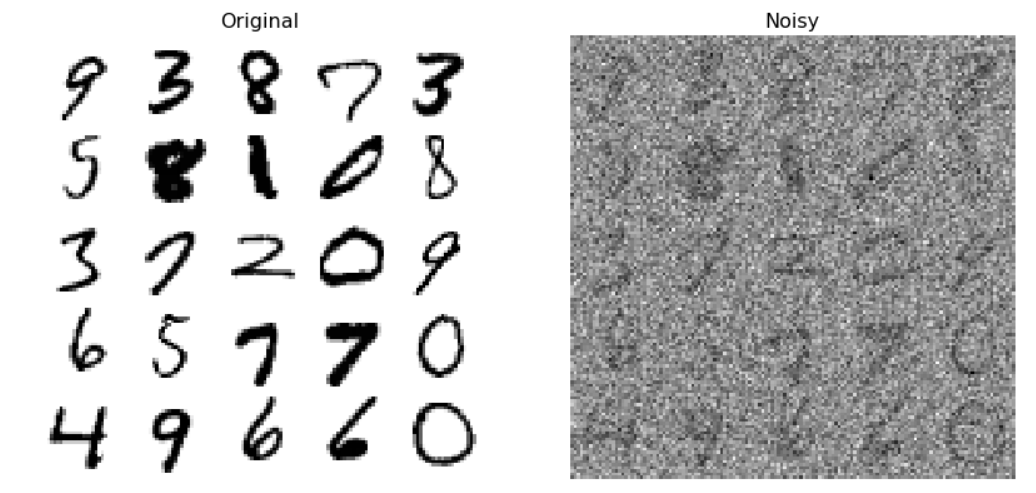
\includegraphics[width=0.7\textwidth]{les8-noisy-numbers}
    \caption{Noise added to original MNIST data.}
    \label{fig:les8-com-c}
\end{figure}

\begin{pyminted}
from sklearn.linear_model import SGDClassifier
clf = RandomForestClassifier(random_state=42)
clf.fit(X_noisy_train, y_noisy_train)
print("Without PCA: ", clf.score(X_noisy_test, y_noisy_test))
\end{pyminted}
\begin{pyconsole}
Without PCA:  0.318
\end{pyconsole}

Using RandomForestClassifier by itself is not very effective. Therefore we will try to achieve a higher score by using compression to reduce the noice.

\begin{pyminted}
from sklearn.pipeline import Pipeline
pipe = Pipeline([
    ("pca", PCA(random_state=42)),
    ("clf", RandomForestClassifier(random_state=42))
])

param_grid = [{
    "pca__n_components": [0.094, 0.095, 0.096, 0.097, 0.098]
}]
\end{pyminted}

The right amount of n\_components can be found by iteratively running a grid search and checking which values comes the closest to have the best fit.

\begin{pyminted}
from sklearn.model_selection import GridSearchCV

search = GridSearchCV(pipe, param_grid, cv=3)
search.fit(X_noisy_train, y_noisy_train)
print(search.best_params_)
\end{pyminted}
\begin{pyconsole}
{'pca__n_components': 0.097}
\end{pyconsole}

The best fit has been found. We will now reuse the value to find the new score and plot it.

\begin{pyminted}
from sklearn.model_selection import train_test_split

pca = PCA(n_components=0.097, random_state=42)
clf = RandomForestClassifier(random_state=42)

X_reduced = pca.fit_transform(X_noisy)
X_recovered = pca.inverse_transform(X_reduced) 
clf.fit(X_recovered, y) % train set her... oh well
print("Classifier with PCA: ", clf.score(X_recovered, y)) % whoops burde nok bruge et test set her
\end{pyminted}
\begin{pyconsole}
Classifier with PCA:  0.9968714285714285
\end{pyconsole}
\begin{pyminted}
plt.figure(figsize=(14, 8))
plt.subplot(121)
plot_digits(X_noisy[::2100])
plt.title("Noisy", fontsize=16)
plt.subplot(122)
plot_digits(X_recovered[::2100])
plt.title("Improved by Compressed", fontsize=16)
\end{pyminted}

\begin{figure}[H]
  \centering
    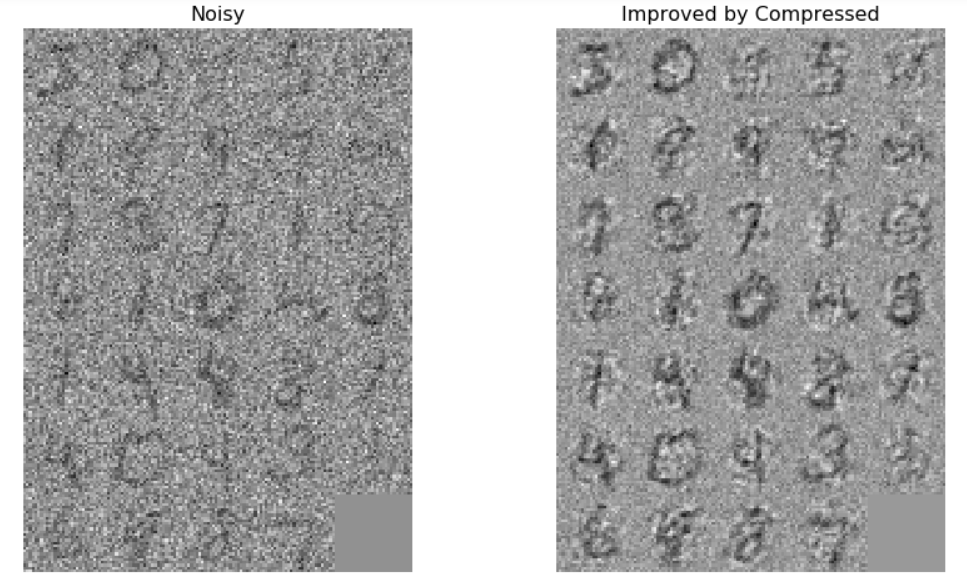
\includegraphics[width=0.7\textwidth]{les8-noisy-compression}
    \caption{Best recovery for the noise.}
    \label{fig:les8-noisy-compression}
\end{figure}

Finally it was possible to identify which parameters for PCA would gain the best recovery. As seen in figure \ref{fig:les8-noisy-compression} it was possible make a recovery of the MNIST dataset which also made it more readable to the human eye. This recovery was quite significant which can be seen by improved classifier score.

\subsection{PCA -> t-SNE features}
The first step when receiving a dataset is to visualize it, and look at potential correlations between features or variables. The MNIST dataset has 784 features. This can be visualized using dimensionality reduction (PCA) and then using t-SNE. t-SNE is mainly intended to be used for visualization of high dimensional data points, and not to extract features. It is good at visualizing clusters, such as it can be seen in the figure. 
\\
Since t-SNE is non parametric, it does not have a way of predicting new data but it can be used to identify clusters, which implies that the data can be modeled as a binary classification. 
\\
t-SNE by itself is very slow when used on the whole data set, so a pipeline with PCA and t-SNE is used  where PCA has 20 components, which is fed into t-SNE that provides 2 components to visualize the data set a seen on figure  \ref{fig:les8-com-c}.

\begin{figure}[H]
  \centering
    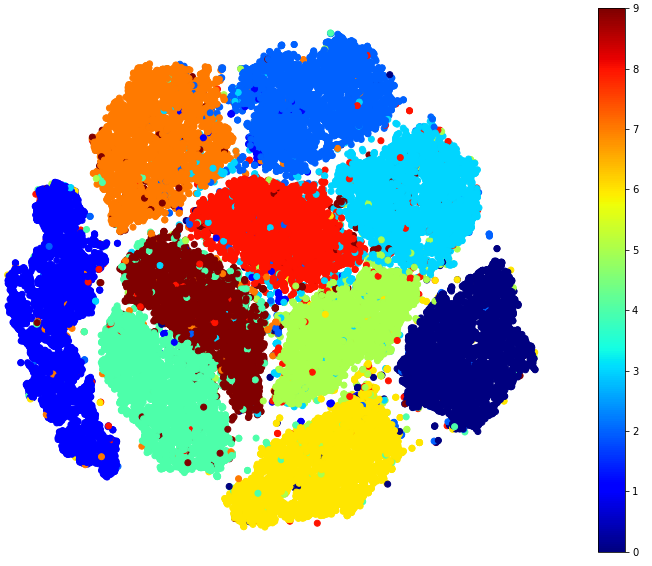
\includegraphics[width=0.7\textwidth]{les8-com-c}
    \caption{PCA -> t-SNE showing the MNIST data set as 10 clusters}
    \label{fig:les8-com-c}
\end{figure}

On figure \ref{fig:les8-com-c} it is clear that the data set can be divided into 10 different  clusters that indicate the values in the MNIST data set. There are some outliers, for example a lot of other colored dots on the red and brown (9 and 8) that are misclassified, which corresponds to the findings from the previous exercises.

\end{document}